%% Responsable : Matias Courderier 

\chapter{Linea Time Reversal (Matias Courdurier. Leonardo Jofr\'e)}

\section{Resumen Estimaci\'on y Clasificaci\'on de Fuentes}

Se propone una reconstrucci\'on de las fuentes s\'{\i}smicas,
como una fuerza, a partir de las mediciones s\'{\i}smicas. Luego se propone
una clasificaci\'on de las fuentes reconstruidas, separ\'andolas en fuentes
contenidas principalmente en un plano o fuentes con componentes comparables
en todas las direcciones.

El estudio de las fuentes s\'{\i}smicas se realiza con la intenci\'on de identificar
propiedades que permitan caracterizar fuentes s\'{\i}smicas cercanas a la superficie
de quiebre. Lograr esta caracterizaci\'on permitir\'{\i}a ocupar la localizci\'on de las
fuentes s\'{\i}smicas para ubicar la superficie de quiebre.

\section{Casos de Estudio}

\subsection{Estimaci\'on de las Fuentes}

Para la lista de eventos
\begin{verbatim}
    '1998_aug_02_07_30_40.d5g'
    '1998_aug_07_16_24_33.i6b'
    '1998_aug_09_21_49_22.4n3'
    '1998_aug_10_07_42_08.2l6'
    '1998_aug_20_08_37_39.ery'
    '1998_jul_04_13_49_28.6bt'
    '1998_jul_05_02_34_05.5hj'
    '1998_jul_06_12_14_55.e8j'
    '1998_jun_26_10_12_59.2ia'
    '1998_jun_27_06_14_09.2jt'
    '1998_jun_28_12_21_02.exs'
    '1998_jun_29_22_24_21.jp6'
    '1998_nov_01_22_40_34.7rv'
    '1998_nov_02_14_15_20.j34'
    '1998_nov_07_21_23_08.ji5'
    '1998_nov_13_06_30_43.00d'
    '1998_oct_10_16_00_15.fzn'
    '1998_oct_15_22_38_44.11n'
    '1998_oct_20_16_06_43.byq'
    '1998_oct_21_17_20_29.8mp'
    '1998_oct_21_18_22_44.h9e'
    '1998_oct_21_20_10_32.kxv'
    '1998_oct_27_19_38_10.1o0'
    '1998_oct_29_18_22_05.2ph'
    '2011_apr_10_02_27'
    '2011_apr_10_04_56'
    '2011_apr_10_06_00'
    '2011_apr_10_06_16'
    '2011_apr_10_07_52'
\end{verbatim}
realizamos la reconstrucci\'on de
las fuentes s\'{\i}smicas como una fuerza
mediante un m\'etodo de m\'{\i}nimos cuadrados descrito m\'as adelante.

\subsection{Input}

Para cada evento se usó el archivo procesado en python con el mismo nombre del
evento.
Estos archivos contienen la posición y el tiempo estimado del evento s\'{\i}smico, y
además una serie de datos importantes, como por ejemplo, la frecuencia de
muestreo de cada uno de los sensores. El detalle se puede ver en el siguiente
ejemplo del primer evento de la lista como objeto matlab.
\begin{verbatim}
               name: {'1998_aug_02_07_30_40.d5g'}
           beta_est: 3500
          alpha_est: 5600
          alpha_ind: []
           beta_ind: []
                gss: [1x7 Geosensor]
              alpha: 5600
               beta: 3500
                rho: 2700
         first_time: 40.5227
          last_time: 41.5579
              count: 7
               LocR: [1x3 double]
        origin_time: 40.5655
           tail_per: 0
              error: 0.0196
                 xi: -892.7790
                 xf: -20.2270
                 yi: -1.5404e+03
                 yf: -715.6420
                 zi: -2.2857e+03
                 zf: -1.9726e+03
                 dx: 14.7890
                 dy: 13.9790
                 dz: 34.7967
                 dt: []
                 nx: []
                 ny: []
                 nz: []
                 nt: []
            n_rsmpl: []
           max_norm: []
             x_axis: [1x60 double]
             y_axis: [1x60 double]
             z_axis: [1x10 double]
             t_axis: [1x50 double]
           X_domain: []
           Y_domain: []
           Z_domain: []
           T_domain: []
    origin_time_est: 40.5655
           LocR_est: [1x3 double]
                 r0: []
            all_est: []
     alpha_ind_post: []
      beta_ind_post: []
                src: [100x4 double]
            filtsrc: [100x4 double]
                  e: []
                 v1: 0.4784
                 v2: 0.2860
                 v3: 0.2356
                vr1: 0.1808
                vr2: 0.2440
                vr3: 0.5752
                  A: []
                  U: [1x73395 double]
            indices: []
             alphas: []
\end{verbatim}
cada evento tiene un conjunto de sensores que pueden ser velocímetros o
acelerómetros. A modo de ejemplo se muestran a continuación el gráfico de cada
una de las mediciones que contiene el evento 1998\_aug\_02\_07\_30\_40.d5g.
 \begin{figure}[H]
\includegraphics[width=0.9\textwidth,height=0.4\textheight]{linea_timerev/figuras/plotSensor(Ev(1),1).pdf}
\caption{Campo de velocidad del sensor 1}
\end{figure}
\begin{figure}[H]
\includegraphics[width=0.9\textwidth,height=0.4\textheight]{linea_timerev/figuras/plotSensor(Ev(1),2).pdf}
\caption{Campo de velocidad del sensor 2}
\end{figure}
\begin{figure}[H]
\includegraphics[width=0.9\textwidth,height=0.4\textheight]{linea_timerev/figuras/plotSensor(Ev(1),3).pdf}
\caption{Campo de velocidad del sensor 3}
\end{figure}
\begin{figure}[H]
\includegraphics[width=0.9\textwidth,height=0.4\textheight]{linea_timerev/figuras/plotSensor(Ev(1),4).pdf}
\caption{Campo de velocidad del sensor 4}
\end{figure}
\begin{figure}[H]
\includegraphics[width=0.9\textwidth,height=0.4\textheight]{linea_timerev/figuras/plotSensor(Ev(1),5).pdf}
\caption{Campo de velocidad del sensor 5}
\end{figure}
\begin{figure}[H]
\includegraphics[width=0.9\textwidth,height=0.4\textheight]{linea_timerev/figuras/plotSensor(Ev(1),6).pdf}
\caption{Campo de velocidad del sensor 6}
\end{figure}
\begin{figure}[H]
\includegraphics[width=0.9\textwidth,height=0.4\textheight]{linea_timerev/figuras/plotSensor(Ev(1),7).pdf}
\caption{Campo de velocidad del sensor 7}
\end{figure}


\subsection{Output}

El algoritmo retorna una estimación de la fuente como una fuerza para cada uno de
los eventos sismicos. La linea vertical roja representa el tiempo estimado por
codelco mediante la variable origin\_time y el número entre $0$ y $1$ bajo
cada gráfico representa la cantidad de fuerza en cada eje, esto quiere decir,
en la componente $x,y,z$ respectivamente.

\begin{figure}[H]
\includegraphics[width=0.9\textwidth,height=0.4\textheight]{linea_timerev/figuras/plotSrcEv1src.pdf}
\caption{Estimación por mínimos cuadrados de la fuente como una fuerza para el
evento 1998\_aug\_02\_07\_30\_40.d5g}
\end{figure}
\begin{figure}[H]
\includegraphics[width=0.9\textwidth,height=0.4\textheight]{linea_timerev/figuras/plotSrcEv2src.pdf}
\caption{Estimación por mínimos cuadrados de la fuente como una fuerza para el
evento 1998\_aug\_07\_16\_24\_33.i6b}
\end{figure}
\begin{figure}[H]
\includegraphics[width=0.9\textwidth,height=0.4\textheight]{linea_timerev/figuras/plotSrcEv3src.pdf}
\caption{Estimación por mínimos cuadrados de la fuente como una fuerza para el
evento 1998\_aug\_09\_21\_49\_22.4n3}
\end{figure}
\begin{figure}[H]
\includegraphics[width=0.9\textwidth,height=0.4\textheight]{linea_timerev/figuras/plotSrcEv4src.pdf}
\caption{Estimación por mínimos cuadrados de la fuente como una fuerza para el
evento 1998\_aug\_10\_07\_42\_08.2l6}
\end{figure}
\begin{figure}[H]
\includegraphics[width=0.9\textwidth,height=0.4\textheight]{linea_timerev/figuras/plotSrcEv5src.pdf}
\caption{Estimación por mínimos cuadrados de la fuente como una fuerza para el
evento 1998\_aug\_20\_08\_37\_39.ery}
\end{figure}
\begin{figure}[H]
\includegraphics[width=0.9\textwidth,height=0.4\textheight]{linea_timerev/figuras/plotSrcEv6src.pdf}
\caption{Estimación por mínimos cuadrados de la fuente como una fuerza para el
evento 1998\_jul\_04\_13\_49\_28.6bt}
\end{figure}
\begin{figure}[H]
\includegraphics[width=0.9\textwidth,height=0.4\textheight]{linea_timerev/figuras/plotSrcEv7src.pdf}
\caption{Estimación por mínimos cuadrados de la fuente como una fuerza para el
evento 1998\_jul\_05\_02\_34\_05.5hj}
\end{figure}
\begin{figure}[H]
\includegraphics[width=0.9\textwidth,height=0.4\textheight]{linea_timerev/figuras/plotSrcEv8src.pdf}
\caption{Estimación por mínimos cuadrados de la fuente como una fuerza para el
evento 1998\_jul\_06\_12\_14\_55.e8j}
\end{figure}
\begin{figure}[H]
\includegraphics[width=0.9\textwidth,height=0.4\textheight]{linea_timerev/figuras/plotSrcEv9src.pdf}
\caption{Estimación por mínimos cuadrados de la fuente como una fuerza para el
evento 1998\_jun\_26\_10\_12\_59.2ia}
\end{figure}
\begin{figure}[H]
\includegraphics[width=0.9\textwidth,height=0.4\textheight]{linea_timerev/figuras/plotSrcEv10src.pdf}
\caption{Estimación por mínimos cuadrados de la fuente como una fuerza para el
evento 1998\_jun\_27\_06\_14\_09.2jt}
\end{figure}
\begin{figure}[H]
\includegraphics[width=0.9\textwidth,height=0.4\textheight]{linea_timerev/figuras/plotSrcEv11src.pdf}
\caption{Estimación por mínimos cuadrados de la fuente como una fuerza para el
evento 1998\_jun\_28\_12\_21\_02.exs}
\end{figure}
\begin{figure}[H]
\includegraphics[width=0.9\textwidth,height=0.4\textheight]{linea_timerev/figuras/plotSrcEv12src.pdf}
\caption{Estimación por mínimos cuadrados de la fuente como una fuerza para el
evento 1998\_jun\_29\_22\_24\_21.jp6}
\end{figure}
\begin{figure}[H]
\includegraphics[width=0.9\textwidth,height=0.4\textheight]{linea_timerev/figuras/plotSrcEv13src.pdf}
\caption{Estimación por mínimos cuadrados de la fuente como una fuerza para el
evento 1998\_nov\_01\_22\_40\_34.7rv}
\end{figure}
\begin{figure}[H]
\includegraphics[width=0.9\textwidth,height=0.4\textheight]{linea_timerev/figuras/plotSrcEv14src.pdf}
\caption{Estimación por mínimos cuadrados de la fuente como una fuerza para el
evento 1998\_nov\_02\_14\_15\_20.j34}
\end{figure}
\begin{figure}[H]
\includegraphics[width=0.9\textwidth,height=0.4\textheight]{linea_timerev/figuras/plotSrcEv15src.pdf}
\caption{Estimación por mínimos cuadrados de la fuente como una fuerza para el
evento 1998\_nov\_07\_21\_23\_08.ji5}
\end{figure}
\begin{figure}[H]
\includegraphics[width=0.9\textwidth,height=0.4\textheight]{linea_timerev/figuras/plotSrcEv16src.pdf}
\caption{Estimación por mínimos cuadrados de la fuente como una fuerza para el
evento 1998\_nov\_13\_06\_30\_43.00d}
\end{figure}
\begin{figure}[H]
\includegraphics[width=0.9\textwidth,height=0.4\textheight]{linea_timerev/figuras/plotSrcEv17src.pdf}
\caption{Estimación por mínimos cuadrados de la fuente como una fuerza para el
evento 1998\_oct\_10\_16\_00\_15.fzn}
\end{figure}
\begin{figure}[H]
\includegraphics[width=0.9\textwidth,height=0.4\textheight]{linea_timerev/figuras/plotSrcEv18src.pdf}
\caption{Estimación por mínimos cuadrados de la fuente como una fuerza para el
evento 1998\_oct\_15\_22\_38\_44.11n}
\end{figure}
\begin{figure}[H]
\includegraphics[width=0.9\textwidth,height=0.4\textheight]{linea_timerev/figuras/plotSrcEv19src.pdf}
\caption{Estimación por mínimos cuadrados de la fuente como una fuerza para el
evento 1998\_oct\_20\_16\_06\_43.byq}
\end{figure}
\begin{figure}[H]
\includegraphics[width=0.9\textwidth,height=0.4\textheight]{linea_timerev/figuras/plotSrcEv20src.pdf}
\caption{Estimación por mínimos cuadrados de la fuente como una fuerza para el
evento 1998\_oct\_21\_17\_20\_29.8mp}
\end{figure}
\begin{figure}[H]
\includegraphics[width=0.9\textwidth,height=0.4\textheight]{linea_timerev/figuras/plotSrcEv21src.pdf}
\caption{Estimación por mínimos cuadrados de la fuente como una fuerza para el
evento 1998\_oct\_21\_18\_22\_44.h9e}
\end{figure}
\begin{figure}[H]
\includegraphics[width=0.9\textwidth,height=0.4\textheight]{linea_timerev/figuras/plotSrcEv22src.pdf}
\caption{Estimación por mínimos cuadrados de la fuente como una fuerza para el
evento 1998\_oct\_21\_20\_10\_32.kxv}
\end{figure}
\begin{figure}[H]
\includegraphics[width=0.9\textwidth,height=0.4\textheight]{linea_timerev/figuras/plotSrcEv23src.pdf}
\caption{Estimación por mínimos cuadrados de la fuente como una fuerza para el
evento 1998\_oct\_27\_19\_38\_10.1o0}
\end{figure}
\begin{figure}[H]
\includegraphics[width=0.9\textwidth,height=0.4\textheight]{linea_timerev/figuras/plotSrcEv24src.pdf}
\caption{Estimación por mínimos cuadrados de la fuente como una fuerza para el
evento 1998\_oct\_29\_18\_22\_05.2ph}
\end{figure}
\begin{figure}[H]
\includegraphics[width=0.9\textwidth,height=0.4\textheight]{linea_timerev/figuras/plotSrcEv25src.pdf}
\caption{Estimación por mínimos cuadrados de la fuente como una fuerza para el
evento 2011\_apr\_10\_02\_27}
\end{figure}
\begin{figure}[H]
\includegraphics[width=0.9\textwidth,height=0.4\textheight]{linea_timerev/figuras/plotSrcEv26src.pdf}
\caption{Estimación por mínimos cuadrados de la fuente como una fuerza para el
evento 2011\_apr\_10\_04\_56}
\end{figure}
\begin{figure}[H]
\includegraphics[width=0.9\textwidth,height=0.4\textheight]{linea_timerev/figuras/plotSrcEv27src.pdf}
\caption{Estimación por mínimos cuadrados de la fuente como una fuerza para el
evento 2011\_apr\_10\_06\_00}
\end{figure}
\begin{figure}[H]
\includegraphics[width=0.9\textwidth,height=0.4\textheight]{linea_timerev/figuras/plotSrcEv28src.pdf}
\caption{Estimación por mínimos cuadrados de la fuente como una fuerza para el
evento 2011\_apr\_10\_06\_16}
\end{figure}
\begin{figure}[H]
\includegraphics[width=0.9\textwidth,height=0.4\textheight]{linea_timerev/figuras/plotSrcEv29src.pdf}
\caption{Estimación por mínimos cuadrados de la fuente como una fuerza para el
evento 2011\_apr\_10\_07\_52}
\end{figure}

\section{Test de Reconstrucci\'on de Fuentes}

Para validar que la reconstrucción de las fuentes sísmicas de cada uno de los
eventos es correcta, se diseño un test en el cual mediante una fuente artificial
se generan sensores artificiales en las mismas posiciones de las de un evento
real. Luego se reconstruye la fuente mediante mínimos cuadrados y se compara con
la fuente artificial.

Para el evento 1998\_aug\_02\_07\_30\_40.d5g se obtuvieron los siguientes
resultados que validan el funcionamiento del software.

\begin{figure}[H]
\centering
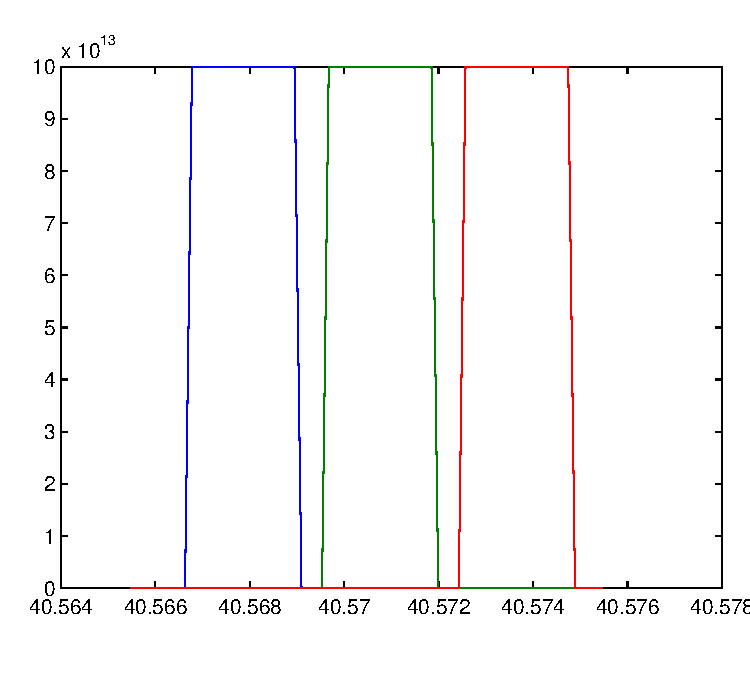
\includegraphics[width=0.5\textwidth,height=0.4\textheight]{linea_timerev/figuras/testRec/artsrc.pdf}
\caption{Fuente artificial para el evento 1998\_aug\_02\_07\_30\_40.d5g}
\end{figure}

\begin{figure}[H]
\centering
\includegraphics[width=0.5\textwidth,height=0.4\textheight]{linea_timerev/figuras/testRec/recartsrc.pdf}
\caption{Reconstrucción de la fuente artificial para el evento
1998\_aug\_02\_07\_30\_40.d5g}
\end{figure}

\begin{figure}[H]
\centering
\includegraphics[width=0.5\textwidth,height=0.4\textheight]{linea_timerev/figuras/testRec/bothtestsrc.pdf}
\caption{Superposición entre la fuente artificial y su reconstrucción
1998\_aug\_02\_07\_30\_40.d5g}
\end{figure}


\subsection{Clasificaci\'on de las Fuentes}

El segundo paso consiste en la clasificaci\'on de las fuentes s\'{\i}smicas reconstruidas.
La clasificaci\'on propuesta es separar las fuentes s\'{\i}smicas de acuerdo a si son
fuerzas contenidas en un plano o si son fuerzas con componentes
comparables en todas las direcciones.

En resumen, separaramos las fuentes de acuerdo a la componente m\'as peque\~na,
despu\'es de un proceso de filtrado y rotaci\'on (cambio de base).

\subsection{Output}

Para cada una de las fuentes reconstruidas, el filtrado y rotaci\'on de \'estas, en
componentes principales, entrega los siguientes resultados.

\begin{figure}[H]
\includegraphics[width=0.9\textwidth,height=0.4\textheight]{linea_timerev/figuras/plotSrcEv1filtrotsrc.pdf}
\caption{Filtro y rotación de la fuente como una fuerza para el
evento 1998\_aug\_02\_07\_30\_40.d5g}
\end{figure}
\begin{figure}[H]
\includegraphics[width=0.9\textwidth,height=0.4\textheight]{linea_timerev/figuras/plotSrcEv2filtrotsrc.pdf}
\caption{Filtro y rotación de la fuente estimada como una fuerza para el
evento 1998\_aug\_07\_16\_24\_33.i6b}
\end{figure}
\begin{figure}[H]
\includegraphics[width=0.9\textwidth,height=0.4\textheight]{linea_timerev/figuras/plotSrcEv3filtrotsrc.pdf}
\caption{Filtro y rotación de la fuente estimada como una fuerza para el
evento 1998\_aug\_09\_21\_49\_22.4n3}
\end{figure}
\begin{figure}[H]
\includegraphics[width=0.9\textwidth,height=0.4\textheight]{linea_timerev/figuras/plotSrcEv4filtrotsrc.pdf}
\caption{Filtro y rotación de la fuente estimada como una fuerza para el
evento 1998\_aug\_10\_07\_42\_08.2l6}
\end{figure}
\begin{figure}[H]
\includegraphics[width=0.9\textwidth,height=0.4\textheight]{linea_timerev/figuras/plotSrcEv5filtrotsrc.pdf}
\caption{Filtro y rotación de la fuente estimada como una fuerza para el
evento 1998\_aug\_20\_08\_37\_39.ery}
\end{figure}
\begin{figure}[H]
\includegraphics[width=0.9\textwidth,height=0.4\textheight]{linea_timerev/figuras/plotSrcEv6filtrotsrc.pdf}
\caption{Filtro y rotación de la fuente estimada como una fuerza para el
evento 1998\_jul\_04\_13\_49\_28.6bt}
\end{figure}
\begin{figure}[H]
\includegraphics[width=0.9\textwidth,height=0.4\textheight]{linea_timerev/figuras/plotSrcEv7filtrotsrc.pdf}
\caption{Filtro y rotación de la fuente estimada como una fuerza para el
evento 1998\_jul\_05\_02\_34\_05.5hj}
\end{figure}
\begin{figure}[H]
\includegraphics[width=0.9\textwidth,height=0.4\textheight]{linea_timerev/figuras/plotSrcEv8filtrotsrc.pdf}
\caption{Filtro y rotación de la fuente estimada como una fuerza para el
evento 1998\_jul\_06\_12\_14\_55.e8j}
\end{figure}
\begin{figure}[H]
\includegraphics[width=0.9\textwidth,height=0.4\textheight]{linea_timerev/figuras/plotSrcEv9filtrotsrc.pdf}
\caption{Filtro y rotación de la fuente estimada como una fuerza para el
evento 1998\_jun\_26\_10\_12\_59.2ia}
\end{figure}
\begin{figure}[H]
\includegraphics[width=0.9\textwidth,height=0.4\textheight]{linea_timerev/figuras/plotSrcEv10filtrotsrc.pdf}
\caption{Filtro y rotación de la fuente estimada como una fuerza para el
evento 1998\_jun\_27\_06\_14\_09.2jt}
\end{figure}
\begin{figure}[H]
\includegraphics[width=0.9\textwidth,height=0.4\textheight]{linea_timerev/figuras/plotSrcEv11filtrotsrc.pdf}
\caption{Filtro y rotación de la fuente estimada como una fuerza para el
evento 1998\_jun\_28\_12\_21\_02.exs}
\end{figure}
\begin{figure}[H]
\includegraphics[width=0.9\textwidth,height=0.4\textheight]{linea_timerev/figuras/plotSrcEv12filtrotsrc.pdf}
\caption{Filtro y rotación de la fuente estimada como una fuerza para el
evento 1998\_jun\_29\_22\_24\_21.jp6}
\end{figure}
\begin{figure}[H]
\includegraphics[width=0.9\textwidth,height=0.4\textheight]{linea_timerev/figuras/plotSrcEv13filtrotsrc.pdf}
\caption{Filtro y rotación de la fuente estimada como una fuerza para el
evento 1998\_nov\_01\_22\_40\_34.7rv}
\end{figure}
\begin{figure}[H]
\includegraphics[width=0.9\textwidth,height=0.4\textheight]{linea_timerev/figuras/plotSrcEv14filtrotsrc.pdf}
\caption{Filtro y rotación de la fuente estimada como una fuerza para el
evento 1998\_nov\_02\_14\_15\_20.j34}
\end{figure}
\begin{figure}[H]
\includegraphics[width=0.9\textwidth,height=0.4\textheight]{linea_timerev/figuras/plotSrcEv15filtrotsrc.pdf}
\caption{Filtro y rotación de la fuente estimada como una fuerza para el
evento 1998\_nov\_07\_21\_23\_08.ji5}
\end{figure}
\begin{figure}[H]
\includegraphics[width=0.9\textwidth,height=0.4\textheight]{linea_timerev/figuras/plotSrcEv16filtrotsrc.pdf}
\caption{Filtro y rotación de la fuente estimada como una fuerza para el
evento 1998\_nov\_13\_06\_30\_43.00d}
\end{figure}
\begin{figure}[H]
\includegraphics[width=0.9\textwidth,height=0.4\textheight]{linea_timerev/figuras/plotSrcEv17filtrotsrc.pdf}
\caption{Filtro y rotación de la fuente estimada como una fuerza para el
evento 1998\_oct\_10\_16\_00\_15.fzn}
\end{figure}
\begin{figure}[H]
\includegraphics[width=0.9\textwidth,height=0.4\textheight]{linea_timerev/figuras/plotSrcEv18filtrotsrc.pdf}
\caption{Filtro y rotación de la fuente estimada como una fuerza para el
evento 1998\_oct\_15\_22\_38\_44.11n}
\end{figure}
\begin{figure}[H]
\includegraphics[width=0.9\textwidth,height=0.4\textheight]{linea_timerev/figuras/plotSrcEv19filtrotsrc.pdf}
\caption{Filtro y rotación de la fuente estimada como una fuerza para el
evento 1998\_oct\_20\_16\_06\_43.byq}
\end{figure}
\begin{figure}[H]
\includegraphics[width=0.9\textwidth,height=0.4\textheight]{linea_timerev/figuras/plotSrcEv20filtrotsrc.pdf}
\caption{Filtro y rotación de la fuente estimada como una fuerza para el
evento 1998\_oct\_21\_17\_20\_29.8mp}
\end{figure}
\begin{figure}[H]
\includegraphics[width=0.9\textwidth,height=0.4\textheight]{linea_timerev/figuras/plotSrcEv21filtrotsrc.pdf}
\caption{Filtro y rotación de la fuente estimada como una fuerza para el
evento 1998\_oct\_21\_18\_22\_44.h9e}
\end{figure}
\begin{figure}[H]
\includegraphics[width=0.9\textwidth,height=0.4\textheight]{linea_timerev/figuras/plotSrcEv22filtrotsrc.pdf}
\caption{Filtro y rotación de la fuente estimada como una fuerza para el
evento 1998\_oct\_21\_20\_10\_32.kxv}
\end{figure}
\begin{figure}[H]
\includegraphics[width=0.9\textwidth,height=0.4\textheight]{linea_timerev/figuras/plotSrcEv23filtrotsrc.pdf}
\caption{Filtro y rotación de la fuente estimada como una fuerza para el
evento 1998\_oct\_27\_19\_38\_10.1o0}
\end{figure}
\begin{figure}[H]
\includegraphics[width=0.9\textwidth,height=0.4\textheight]{linea_timerev/figuras/plotSrcEv24filtrotsrc.pdf}
\caption{Filtro y rotación de la fuente estimada como una fuerza para el
evento 1998\_oct\_29\_18\_22\_05.2ph}
\end{figure}
\begin{figure}[H]
\includegraphics[width=0.9\textwidth,height=0.4\textheight]{linea_timerev/figuras/plotSrcEv25filtrotsrc.pdf}
\caption{Filtro y rotación de la fuente estimada como una fuerza para el
evento 2011\_apr\_10\_02\_27}
\end{figure}
\begin{figure}[H]
\includegraphics[width=0.9\textwidth,height=0.4\textheight]{linea_timerev/figuras/plotSrcEv26filtrotsrc.pdf}
\caption{Filtro y rotación de la fuente estimada como una fuerza para el
evento 2011\_apr\_10\_04\_56}
\end{figure}
\begin{figure}[H]
\includegraphics[width=0.9\textwidth,height=0.4\textheight]{linea_timerev/figuras/plotSrcEv27filtrotsrc.pdf}
\caption{Filtro y rotación de la fuente estimada como una fuerza para el
evento 2011\_apr\_10\_06\_00}
\end{figure}
\begin{figure}[H]
\includegraphics[width=0.9\textwidth,height=0.4\textheight]{linea_timerev/figuras/plotSrcEv28filtrotsrc.pdf}
\caption{Filtro y rotación de la fuente estimada como una fuerza para el
evento 2011\_apr\_10\_06\_16}
\end{figure}
\begin{figure}[H]
\includegraphics[width=0.9\textwidth,height=0.4\textheight]{linea_timerev/figuras/plotSrcEv29filtrotsrc.pdf}
\caption{Filtro y rotación de la fuente estimada como una fuerza para el
evento 2011\_apr\_10\_07\_52}
\end{figure}

\section{Conclusi\'on Estimaci\'on y Clasificaci\'on de Fuentes}

Al considerar las 29 fuentes s\'{\i}smicas reconstruidas, los valores
obtenidos para  las componentes m\'as peque\~nas (despu\'es del filtrado y la
rotaci\'on) son:

\begin{figure}[H]
\centerline{\includegraphics[width=0.5\textwidth]{linea_timerev/figuras/clasificacion.pdf}}
\caption{Grafico con la clasificación de la componente más pequeña mediante
algoritmo de las kmedias con 3 clusters}
\end{figure}

El valor para estas cantidades varia entre 0 y 1/3. Valores
cercanos a 0 corresponden a fuentes contenidas principalmente
en un plano, valores cercanos a 1/3 corresponde a fuentes
con componentes comparables en todas las direcciones.

Al estudiar las 29 fuentes reconstruidas se observa
acumulamiento de las primeras componentes en tres grupos.
Aquellos sismos con primera componente por debajo
de 0.165, sismos con primera componente entre 0.165
y 0.22 y sismos con primera componente mayor a 0.22.
Esta diferenciaci\'on se observa claramente en el
grupo de eventos considerados, que ya es de un tama\~no
razonable, pero se sugiere validar la observaci\'on
estudiando un conjunto m\'as grande de eventos. La
diferenciaci\'on observada confirma en primera instancia, de
manera muy positiva, la posibilidad de clasificar
los eventos de acuerdo a su componente m\'as peque\~na.

Esto, en particular, se puede ocupar como informaci\'on
complementaria para la clasificaci\'on utilizada en la linea s\'{\i}smica
de este proyecto.

\section{Resumen Time-reversal}

En time-reversal se calcula la propagaci\'on de una onda cuyas fuentes se relacionan
con las mediciones sismogr\'aficas invertidas en el tiempo. En el caso ideal de suficientes
mediciones, adecuadamente distribuidas, la onda as\'{\i} generada deber\'{\i}a
concentrarse en la posici\'on correspondiente al or\'{\i}gen del sismo y dar indicaciones
del tiempo de origen y la forma de la fuente.

\section{Casos de Estudio}

Los casos de estudio son los siguentes $3$ eventos:

\begin{verbatim}
    '1998_aug_02_07_30_40.d5g'
    '1998_aug_07_16_24_33.i6b'
    '1998_aug_09_21_49_22.4n3'
\end{verbatim}



\subsection{Input}

Set de datos entregados por codelco, procesados por el script en python y
consumidos por matlab mediante el script de importación.

\subsection{Output}
 Se obtienen las siguientes visualizaciones de las inversiones de los campos de
 desplazamiento de las ondas sísmicas.
 
\begin{figure}[H]
\begin{tabular}{ccc}
	\includegraphics[width=0.3\textwidth]{linea_timerev/figuras/timereversal/ev1/tr124.png}&
	\includegraphics[width=0.3\textwidth]{linea_timerev/figuras/timereversal/ev1/tr125.png}&
	\includegraphics[width=0.3\textwidth]{linea_timerev/figuras/timereversal/ev1/tr126.png}\\
	\includegraphics[width=0.3\textwidth]{linea_timerev/figuras/timereversal/ev1/tr127.png}&
	\includegraphics[width=0.3\textwidth]{linea_timerev/figuras/timereversal/ev1/tr128.png}&
	\includegraphics[width=0.3\textwidth]{linea_timerev/figuras/timereversal/ev1/tr129.png}\\
	\includegraphics[width=0.3\textwidth]{linea_timerev/figuras/timereversal/ev1/tr130.png}&
	\includegraphics[width=0.3\textwidth]{linea_timerev/figuras/timereversal/ev1/tr131.png}&
	\includegraphics[width=0.3\textwidth]{linea_timerev/figuras/timereversal/ev1/tr132.png}\\
	\includegraphics[width=0.3\textwidth]{linea_timerev/figuras/timereversal/ev1/tr133.png}&
	\includegraphics[width=0.3\textwidth]{linea_timerev/figuras/timereversal/ev1/tr134.png}&
	\includegraphics[width=0.3\textwidth]{linea_timerev/figuras/timereversal/ev1/tr135.png}\\
	\includegraphics[width=0.3\textwidth]{linea_timerev/figuras/timereversal/ev1/tr136.png}&
	\includegraphics[width=0.3\textwidth]{linea_timerev/figuras/timereversal/ev1/tr137.png}&
	\includegraphics[width=0.3\textwidth]{linea_timerev/figuras/timereversal/ev1/tr138.png}\\
\end{tabular}
\caption{Time reversal para el evento 1998\_aug\_02\_07\_30\_40.d5g}
\end{figure}

\begin{figure}[H]
\begin{tabular}{ccc}
	\includegraphics[width=0.3\textwidth]{linea_timerev/figuras/timereversal/ev2/tr224.png}&
	\includegraphics[width=0.3\textwidth]{linea_timerev/figuras/timereversal/ev2/tr225.png}&
	\includegraphics[width=0.3\textwidth]{linea_timerev/figuras/timereversal/ev2/tr226.png}\\
	\includegraphics[width=0.3\textwidth]{linea_timerev/figuras/timereversal/ev2/tr227.png}&
	\includegraphics[width=0.3\textwidth]{linea_timerev/figuras/timereversal/ev2/tr228.png}&
	\includegraphics[width=0.3\textwidth]{linea_timerev/figuras/timereversal/ev2/tr229.png}\\
	\includegraphics[width=0.3\textwidth]{linea_timerev/figuras/timereversal/ev2/tr230.png}&
	\includegraphics[width=0.3\textwidth]{linea_timerev/figuras/timereversal/ev2/tr231.png}&
	\includegraphics[width=0.3\textwidth]{linea_timerev/figuras/timereversal/ev2/tr232.png}\\
	\includegraphics[width=0.3\textwidth]{linea_timerev/figuras/timereversal/ev2/tr233.png}&
	\includegraphics[width=0.3\textwidth]{linea_timerev/figuras/timereversal/ev2/tr234.png}&
	\includegraphics[width=0.3\textwidth]{linea_timerev/figuras/timereversal/ev2/tr235.png}\\
	\includegraphics[width=0.3\textwidth]{linea_timerev/figuras/timereversal/ev2/tr236.png}&
	\includegraphics[width=0.3\textwidth]{linea_timerev/figuras/timereversal/ev2/tr237.png}&
	\includegraphics[width=0.3\textwidth]{linea_timerev/figuras/timereversal/ev2/tr238.png}\\
\end{tabular}
\caption{Time reversal para el evento 1998\_aug\_07\_16\_24\_33.i6b}
\end{figure}

\begin{figure}[H]
\begin{tabular}{ccc}
	\includegraphics[width=0.3\textwidth]{linea_timerev/figuras/timereversal/ev3/tr324.png}&
	\includegraphics[width=0.3\textwidth]{linea_timerev/figuras/timereversal/ev3/tr325.png}&
	\includegraphics[width=0.3\textwidth]{linea_timerev/figuras/timereversal/ev3/tr326.png}\\
	\includegraphics[width=0.3\textwidth]{linea_timerev/figuras/timereversal/ev3/tr327.png}&
	\includegraphics[width=0.3\textwidth]{linea_timerev/figuras/timereversal/ev3/tr328.png}&
	\includegraphics[width=0.3\textwidth]{linea_timerev/figuras/timereversal/ev3/tr329.png}\\
	\includegraphics[width=0.3\textwidth]{linea_timerev/figuras/timereversal/ev3/tr330.png}&
	\includegraphics[width=0.3\textwidth]{linea_timerev/figuras/timereversal/ev3/tr331.png}&
	\includegraphics[width=0.3\textwidth]{linea_timerev/figuras/timereversal/ev3/tr332.png}\\
	\includegraphics[width=0.3\textwidth]{linea_timerev/figuras/timereversal/ev3/tr333.png}&
	\includegraphics[width=0.3\textwidth]{linea_timerev/figuras/timereversal/ev3/tr334.png}&
	\includegraphics[width=0.3\textwidth]{linea_timerev/figuras/timereversal/ev3/tr335.png}\\
	\includegraphics[width=0.3\textwidth]{linea_timerev/figuras/timereversal/ev3/tr336.png}&
	\includegraphics[width=0.3\textwidth]{linea_timerev/figuras/timereversal/ev3/tr337.png}&
	\includegraphics[width=0.3\textwidth]{linea_timerev/figuras/timereversal/ev3/tr338.png}\\
\end{tabular}
\caption{Time reversal para el evento 1998\_aug\_09\_21\_49\_22.4n3}
\end{figure}


\section{Conclusiones en Time Reversal}

La implementaci\'on y experimentaci\'on del m\'etodo de time reversal con datos reales
result\'o ser bastante m\'as dif\'{\i}cil que el caso de datos sint\'eticos realizados en
la primera etapa de este proyecto.

Las mayores dificultades aparecieron en dos aspectos independientes
del m\'etodo.

Primero, en t\'erminos de complejidad computacional, el gran tama\~no de las
mediciones (del orden de $4\times10^3$ mediciones temporales por cada sensor
por cada componente) y el tama\~no necesario de la reconstrucci\'on
(del orden de $60\times60\times10$ puntos espaciales, por 50 puntos temporales,
por cada componente) hicieron imposible una implementaci\'on directa del m\'etodo
desarrollado durante la primera etapa.
Para superar esta dificultad, programamos un m\'etodo de subsampleo variable de las
mediciones y cambiamos los m\'etodos de propagaci\'on de onda ya implementados, para
poder trabajar con esta nueva estructura de datos.

Segundo, otra dificultad surgi\'o por la relativamente baja cobertura de sensores. En particular,
en las experimentaciones realizadas
observamos que la baja distribuci\'on de sensores alrededor
de las fuentes s\'{\i}smicas provocaba una sobreponderaci\'on artificial de los
sensores que se encontraban m\'as cerca de la fuente y una sobreponderaci\'on
artificial en las direcciones con mayor densidad de sensores. Corregimos parcialmente
eso con una pre-ponderarci\'on de las mediciones (multiplicando por las distancias
entre sensores y la posici\'on estimada de la fuente al cuadrado, de acuerdo a
 la expresi\'on de la funci\'on de Green). Esto mejor\'o bastante la focalizaci\'on de
la onda de time reversal, pero no pudimos lidiar de manera completa con la distribuci\'on
no homog\'enea de sensores alrededor de la fuente s\'{\i}smica.

En conclusi\'on, para  los eventos estudiados se logr\'o superar bastantes de las dificultades
que se presentaron en el desarrollo del m\'etodo, obteniendo una implementaci\'on de time
reversal con un tiempo de c\'omputo factible (del orden de 90 minutos) y en
la que se observa
focalizaci\'on de la onda de time reversal en la
posici\'on y tiempos adecuados (seg\'un estimaciones independientes de tiempos
de viaje). Pero a pesar de esto, nuestra evaluaci\'on final del m\'etodo es que no
produjo resultados al nivel de las expectativas que ten\'{\i}amos. Las reconstrucci\'ones
obtenidas no presentan suficiente resoluci\'on y estabilidad para una
estimaci\'on robusta de
la posici\'on, tiempo de origen y forma de las fuentes s\'{\i}smicas.


\section{Modelos}

\subsection{Ecuaci\'on de Ondas El\'astica}

Consideraremos que la propagaci\'on de la onda s\'{\i}smica en
el medio rocoso esta bien modelada por la ecuaci\'on de onda
el\'astica en un medio homog\'eneo sin fronteras.
Es decir, si $u(x,y,z,t)$ representa el desplazamiento en el punto
$(x,y,z)$ debido a la onda, en el tiempo $t$, entonces asumimos
que la propagaci\'on de la onda $u$ est\'a modelada adecuadamente
por la ecuaci\'on
\begin{align}\label{eqn:elasticwave}
\rho\frac{\partial^2 u}{\partial t^2}-(\lambda+2\mu)\nabla(\nabla\cdot u)+\mu\nabla\times(\nabla\times u)=F \qquad\textnormal{ en } \quad\R^3
\end{align}
donde la densidad $\rho$ y los par\'ametros de Lam\'e $\lambda,\mu$ se asumen constantes 
y conocidos. El lado derecho $F$ es la fuente (fuerza localizada) del s\'{\i}smo.


Para resolver la ecuaci\'on \eqref{eqn:elasticwave} tenemos una expresi\'on expl\'{\i}cita
de la funci\'on de Green, es decir del campo de desplazamientos en la direcci\'on $i$
debido a un impulso en la direcci\'on $j$ en el tiempo $t=0$ ($i,j\in\{\hat{x},\hat{y},\hat{z}\}$).
Tenemos que $G_i,j=0$ para $t<0$ y para $t\geq0$
$$G_{ij}(x,y,z,t)=
\frac{1}{4\pi\rho}\big(3\gamma_i\gamma_j-\delta_{ij}\big)\frac{t}{r^3}\one_{[\frac{r}{\alpha},\frac{r}{\beta}]}(t)
+\frac{1}{4\pi\rho\alpha^2}\gamma_i\gamma_j\frac{1}{r}\delta(t-\frac{r}{\alpha})
-\frac{1}{4\pi\rho\beta^2}\big(\gamma_i\gamma_j-\delta_{ij}\big)\frac{1}{r}\delta(t-\frac{r}{\beta})$$
donde $r=\sqrt{x^2+y^2+z^2}$, $\gamma_{\hat{x}}=x/r$ (an\'alogo para $i\in\{\hat{y},\hat{z}\}$),
$\delta_{ij}=1$ si $i=j$ y $0$ si $i\neq j$, $\one_A(t)=1$ si $t\in A$ y $0$ si $t\notin A$, $\delta(\cdot)$
es el delta de Dirac en el tiempo (una dimensi\'on) y donde $\alpha=\sqrt{(\lambda+2\mu)/\rho}$ y
$\beta=\sqrt{\mu/\rho}$ son las velocidades de la onda $p$ y $s$ respectivamente.

\subsection{Modelo de Time-Reversal}

La observaci\'on principal que motiva y justifica el m\'etodo de time
reversal es que si $u(x,y,z,t)$ es una soluci\'on de la ecuaci\'on
el\'astica, entonces $\tilde{u}(x,y,z,t)=u(x,y,z,T-t)$ tambi\'en es
una soluci\'on de la ecuaci\'on el\'astica con los {\bf mismos coeficientes}.

Si se mide $u(x,y,z,t)$ en toda la frontera
$\Sigma$ de alg\'un conjunto $\Omega\subset\R^3$, durante un intervalo de
tiempo $[t_1,t_2]$,  se puede resolver la ecuaci\'on
\begin{align*}
\rho\frac{\partial^2 \hat{u}}{\partial t^2}-(\lambda+2\mu)\nabla(\nabla\cdot \hat{u})+\mu\nabla\times(\nabla\times \hat{u})=0\\
\hat{u}(x,y,z,t)=u(x,y,z,t_2-t) \textnormal{ para } (x,y,z)\in\Sigma, t\in[0,t_2-t_1]
\end{align*}

La unicidad de la soluci\'on implica que con condiciones adecuadas $\hat{u}(x,y,z,t)=u(x,y,z,t_2-t)$  en $\Omega$
para todo $t\in[0,t_2-t_0]$, obteniendo $u(x,y,z,t_2-t_0)$ en el momento del s\'{\i}smo
y por ende recuperando la fuente s\'{\i}smica (en principio
$t_0$ no es conocido y tambi\'en debe ser recuperado en este
proceso).

En el m\'etodo de time-reversal se propone invertir el tiempo en las mediciones
 y ocuparlas como fuentes sint\'eticas para producir una onda que se concentre
en la fuente s\'{\i}smica original, recuperando as\'{\i} la posici\'on, el tiempo en
que se origin\'o y la forma de \'esta.

M\'as espec\'{\i}ficamente, la onda $u$ (o derivadas temporales de $u$ que permitir\'{\i}an
recuperar $u$) se mide en $K$ estaciones, localizadas en
$\{r_k\}_{k=1}^K$ (cada $r_k=(x_k,y_k,z_k)$) y por intervalos de tiempos
$[0,T]$ con con $0<t_0$ y $T$ suficientemente grande.
Para cada $k=1,...,K$ resolvemos la ecuacion
\begin{align*}\tag{$P_k$}\label{eqn:Gphonek}
\rho\frac{\partial^2 \hat{u}_k}{\partial t^2}-(\lambda+2\mu)\nabla(\nabla\cdot \hat{u}_k)-\mu\nabla\times(\nabla\times \hat{u}_k)=\delta_{r_k}(r)u(r_k,T-t) \textnormal{ para }  t\geq0
\end{align*}
y definimos $\hat{u}=\sum_{k=1}^K\hat{u}_k$. Si la
cobertura de los ge\'ofonos es suficientemente adecuada respecto al
origen de la fuente s\'{\i}smica, entonces $\hat{u}$ deber\'{\i}a
relacionarse con la propagaci\'on invertida de la onda original
(i.e. $u(x,y,z,T-t)$ ) y la focalizaci\'on de
$\hat{u}$ se podr\'{\i}a utilizar para identificar el momento $t_0$ en que
ocurri\'o el sismo y obtener la forma espacial de
la fuente s\'{\i}smica.

Se puede resolver la ecuaci\'on  \eqref{eqn:Gphonek} ocupando la funci\'on de Green,
que conocemos expl\'{\i}citamente y est\'a descrita arriba.
Si $G=[G_{ij}]_{i,j=1,2,3}$ es la matriz sim\'etrica de $3\times3$ con componentes $G_{ij}$,
entonces $\hat{u}_k(x,y,z,t)$ se puede calcular como
$$\hat{u}_k(x,y,z,t)=\int_0^tG((x,y,z)-r_k,t-\tau)\cdot u(r_k,T-\tau)d\tau$$
(donde $G\cdot u$ es el producto entre una matriz de $3\times3$ y un vector en $\R^3$).
Es decir $\hat{u}_k$ corresponde a la convoluci\'on en el tiempo entre la se\~na  del ge\'ofono localizado
en $r_k$ invertida en el tiempo, y la funci\'on de Green trasladada a $r_k$.

Una vez construida $\hat{u}$ se puede estudiar\'{i}a el momento y la forma en la cual se focaliza, lo que
deber\'{\i}a corresponder al momento y la forma de la fuente s\'{\i}smica.

\subsection{Estimaci\'on de Fuentes Utilizando M\'{\i}nimos Cuadrados.}

Como describimos anteriormente, una fuente s\'{\i}smica
(una fuerza) localizada en $r_0=(x_0,y_0,z_0)$ y modulada
temporalmente seg\'un $s(t)$, se puede incluir en la ecuaci\'on \eqref{eqn:elasticwave}
como un lado derecho de la forma $s(t)\delta_{r_0}(r)$.

Denotando la funci\'on de Green de la ecuaci\'on como $G(r|t)$, podemos
calcular el campo de desplazamiento de la onda en el punto $r=(x,y,z)$ en el tiempo $t$,
como
\begin{align*}
u(r,t)=[G(r-r_0|\cdot)* s(\cdot)](t).
\end{align*}

Las mediciones corresponden (despues de integrar temporalmente si es necesario) al campo de desplazamiento,
a lo largo del tiempo, en las posiciones $\{r_k\}_{k=1}^K$. Es decir, nuestras mediciones corresponde
al conocimiento de $u_k(t):= u(r_k,t)$ para $t$ en un intervalo $T_k\subset\R$.

Asumiendo que la posici\'on $r_0$ de la fuente es conocida (obtenida por ejemplo mediante tiempos de viaje)
y que $s(t)$ esta soportado cerca de un tiempo $t_0$ conocido (tambi\'en obtenido por tiempos de viaje
por ejemplo), queremos plantear un m\'etodo de reconstrucci\'on de $s(t)$ mediante m\'{\i}nimos cuadrados.

Consideremos $\{\varphi_j\}_{j=1}^J$ una familia de funci\'ones linealmente independientes, soportadas
alrededor de $t_0$, que nos permitan describir $s(t)$ aproximadamente. Es decir, consideraremos que
\begin{align*}
s(t)=\sum_{j=1}^J \alpha_j \varphi_j(t), \forall t
\end{align*}
La familia $\{\varphi_j\}_{j=1}^J$ est\'a dada y el objetivo es encontrar $\{\alpha_j\}_{j=1}^J$
a partir de las mediciones. Para esto, seg\'un el modelo de propagaci\'on de onda, tenemos que
$\alpha_j$ deber\'{\i}an cumplir, para todo $k=1,...,K$ y para todo $t\in T_k$, que
\begin{align*}
u_k(t)&=[G(r_k-r_0)*s](t)\\
&=[G(r_k-r_0)*\sum_{j=1}^J \alpha_j \varphi_j](t)\\
&=\sum_{j=1}^J \alpha_j [G(r_k-r_0)* \varphi_j](t).\\
\end{align*}
Encontraremos los valores $\{\alpha_j\}_{j=1}^j$ resolviendo la ecuaci\'on anterior, o escogiendo aquellos
que la se acerquen lo m\'as posible a resolverna. M\'as expl\'{\i}citamente, encontraremos los $\alpha_j$
como 
\begin{align*}
\{\alpha_j\}=\arg\min_{\{\alpha_j\}}\Big(\sum_{k=1}^K \int_{T_k} \Big(u_k(t)-
\sum_{j=1}^J \alpha_j [G(r_k-r_0)* \varphi_j](t)\Big)^2dt\Big)
\end{align*}

Como las mediciones temporales son efectivamente discretas, lo anterior se puede
escribir de manera matricial como
\begin{align*}
\arg\min || u-\alpha\cdot A||^2
\end{align*}
donde $u=(u_k(t))_{k=1,...,K; t\in T_k}$, $\alpha=(\alpha_1,...,\alpha_J)$ y $A=\Big([G(r_k-r_0)* \varphi_j](t)\Big)_{k=1,...,K; t\in T_k;  j=1,...,J}$ escritos de manera adecuada.
El problema anterior es un problema est\'andard de m\'{\i}nimos cuadrados y la soluci\'on (de menor norma en
caso de admitir m\'ultiples minimizantes) se escribe como
\begin{align*}
\hat{\alpha}=u\cdot A^t\cdot (AA^t)^\dagger
\end{align*}
(donde $B^\dagger$ es la pseudo-inversa de Perron cuando $B$ no es invertible). Esto entrega una
reconstrucci\'on de $s(t)$ como
\begin{align*}
\hat{s}(t)=\sum_{j=1}^J \hat{\alpha}^j \varphi_j(t)
\end{align*}

\subsection{Clasificaci\'on de Fuentes Reconstruidas.}

Al tener reconstrucciones de las fuentes s\'{\i}smicas, queremos encontrar
una posible clasificaci\'on de las fuentes seg\'un la
proximidad de \'estas a la superficie de quiebre. Obteniendo as\'i informaci\'on
sobre la posici\'on de la superficie de quiebre.

En la linea s\'{\i}smica del proyecto se presentaron ideas y criterios relacionados
a la superficie de quiebre, para clasificaciones de las fuentes s\'{i}ismicas. Dado
que los investigadores de esa linea entienden mucho mejor que nosotros los
mecanismos geof\'{\i}sicos involucrados en la fractura de la roca, nos dimos la
libertad de tomar prestado uno de los criterios que propusieron, haciendo aqu\'{\i}
expl{\i}cito que la autor\'{i}a de esa idea pertenece a los investigadores de
esa linea. 

B\'asicamente, la idea es separar los s\'{i}smos en aquellos correspondientes
a fracturas de cizalla y en aquellos correspondientes a implosi\'on de roca.

Interpretamos esta caracterizaci\'on como eventos correspondientes a fuentes s\'{\i}smicas
contenidas mayoritariamente en un plano y fuentes s\'{\i}smicas con
componentes comparables en todas las direcciones.

Para poder identificar estos dos casos, encontramos la direcci\'on de
menor proyecci\'on para cada fuente s\'{\i}smica y
calculamos la fracci\'on de la fuerza que se proyecta en esa direcci\'on.
\'Esto se obtiene haciendo un cambio de base de la
fuente reconstruida $s(t)\in \R^3$ sobre los vectores propios de la
matriz $[S_{ij}]_{i,j=1,2,3}$, donde $S_{ij}=\int s_i(t)s_j(t) dt$.

La proyecci\'on de menor componente contiente
entre 0 y 1/3 de la fuerza total. Si la menor componente
es 0 la fuente s\'{\i}smica est\'a contenida en un plano, si la menor componente es 1/3
 la fuente s\'{\i}smica
tiene componentes completamente comparables en todas las direcciones.

Idealmente, un valor l\'{\i}mite para la separaci\'on entre fuentes planas y fuentes isotr\'opicas
aparecer\'a naturalmente al estudiar una familia de eventos s\'{\i}smicos.

\section{Descripción del Software y Manual de Uso}

\subsection{Forma de importar los datos al sistema}
La informacion desde los archivos de texto codificados en ascii se importan por
medio de un script en python. El script toma cada archivo y genera una carpeta
con un nombre y además con el sufijo FOLDER. Consideremos como ejemplo el
archivo de sismograma con el nombre
\subsection{Descripción de estructuras de datos}
Las información de un evento está almacenada en dos clases matlab con los
nombres event.m y geonsensor.m los cuales están relacionados como se muestra en
la figura. 

\subsection{Resumen de implementacion (En Matlab y Python)}

\subsubsection{Scripts en Python}
\paragraph{readFile.py}
Se usa una rutina en python para separar la información desde los documentos de
los geofonos y convertirla a archivos que servirán de imput que funciones matlab
trasnformen la información a objetos matlab.
\paragraph{patterns.py}
Conjunto de patrones con la información necesaria que luego se extraerá mediante
readFile.py.

\subsubsection{Clases Matlab}
\paragraph{Event.m}
Clase que contiene una lista de geosensores y los parámetros de un evento
sísmico específico. Estos son los atributos de los set de datos entregados
por Codelco.
\paragraph{Geonsensor.m}
Clase que contiene la información de cada uno de los geofonos en un evento
específico. 
\subsubsection{Documentación de las Rutinas Principales}

\paragraph{Importar información a matlab}
\begin{itemize}
  \item Archivo: script/importEvents.m
  \item Comando: events = importEvents()
  \item Descripción: Almacena la información desde los archivos tratados por el
  script python readFile.py a una vector de objetos Event en matlab.
  \item input: no recibe parámetros de entrada dado que hace lecturas sobre
  archivos de texto almacenados en disco.
  \item output: event lista de objetos del tipo Event que contienen a todos los
  eventos sísmicos almacenados en la carpeta `./project/data sets`  		 
\end{itemize}


\paragraph{Estimar la fuente sismica de un evento sísmico}
\begin{itemize}
  \item Archivo: script/source.m
  \item Comando: [src, filtsrc, error] = source(event, nSrc, L, por)
  \item Descripción: Estima la fuente como una fuerza $f(t)$ en un intervalo de 
  tiempo de largo $L$ dado el conjunto de sismógrafos del evento
  \textbf{event} con una discretización del dominio con \textbf{nSrc} con una
  fracción \textbf{por} de la fuente antes de \textbf{event.origin\_time} es
  cual es el valor estimado por codelco.
  \item input: 
    \begin{itemize}
    \item event: Objeto del tipo Event el cual representa el sísmico del cual se
    quiere obtener la estimación de la fuente $f(t)$ como una fuerza.
    \item nSrc: número de puntos de la discretización uniforme en el tiempo con
    la cual se va a estimar la fuente.
    \item L: largo de la ventana de tiempo en donde se va a estimar la fuente
    \item por: porcentaje de la ventana de tiempo que está antes del tiempo de
    origen estimado por el documento del evento.
    \end{itemize}
  \item output:
  	\begin{itemize}
  	  \item src: fuente sismica como una fuerza en el punto $r_0$ estimado desde
  	  los valores dados por las mediciones de los geofonos
  	  \item filtsrc: src pero filtrada eliminando los modos bajos
  	  \item error: error de estimación 
  	\end{itemize}
\end{itemize}

\paragraph{script/constructsensor.m}

Deduce la forma de un geofono dada una fuente sísmica
\subsection{Manual de uso}
El uso del programa está descrito en dos archivos matlab distintos, en el 
primero sampletimereversal.m se describe como invertir la señal en tiempo. En el
segundo archivo llamado sampleRecSource.m se describen los pasos para la 
reconstruccion de una fuente sismica a partir de la información de los geofonos 
dados por Codelco.


\begin{verbatim}
%lista de todos los eventos sismicos
events = importEvents()
%mostrar el primero y se vera que las variables de este objeto tienen el mismo
% nombre que las variables utilizadas en los set de datos
event(1)

>>
ans = 

  Event

  Properties:
              name: {'1998_aug_02_07_30_40.d5g'}
           beta_est: 3500
          alpha_est: 5600
          alpha_ind: []
           beta_ind: []
                gss: [1x8 Geosensor]
              alpha: 5600
               beta: 3500
                rho: 2700
         first_time: 40.5227
          last_time: 41.5579
              count: 8
               LocR: [-439.5702 -1.1564e+03 -2.1773e+03]
        origin_time: 40.5655
           tail_per: 0
              error: 0.1500
                 xi: -892.7790
                 xf: -20.2270
                 yi: -1.5404e+03
                 yf: -715.6420
                 zi: -2.2857e+03
                 zf: -1.9726e+03
                 dx: 14.7890
                 dy: 13.9790
                 dz: 34.7967
                 dt: []
                 nx: []
                 ny: []
                 nz: []
                 nt: []
            n_rsmpl: []
           max_norm: []
             x_axis: [1x60 double]
             y_axis: [1x60 double]
             z_axis: [1x10 double]
             t_axis: [1x50 double]
           X_domain: []
           Y_domain: []
           Z_domain: []
           T_domain: []
    origin_time_est: 40.5655
           LocR_est: [-439.5702 -1.1564e+03 -2.1773e+03]
                 r0: []
            all_est: []
     alpha_ind_post: []
      beta_ind_post: []
                src: []
            filtsrc: []
                  e: []
                 v1: []
                 v2: []
                 v3: []
                vr1: []
                vr2: []
                vr3: []
                  A: []
                  U: []
            indices: []
             alphas: []
\end{verbatim}


\subsubsection{Geonsensor.m} 
Clase que contiene los atributos de un geosensor especifico en un evento
sísmico. Contiene las mediciones y propiedades calculadas
necesarias para los algoritmos.
\paragraph{Ejemplo}
\begin{verbatim}
%lista de todos los eventos sismicos
events = importEvents()
%mostrar el primer geosensor de la lista de el evento 1
event(1).gss(1)
ans = 

  Geosensor

  Properties:
                   cuttime: 40.6138
                 firsttime: 40.5286
                  lasttime: 41.0173
       resampleErrorOnNorm: 0.1499
              resampleSize: 191
        timeresamplevector: [1x191 double]
                timevector: [1x4888 double]
        diferenciaPSvalida: 1
         medicionesValidas: [1 1 1]
                        r0: [-369.6930 -1.1323e+03 -2.1262e+03]
    hardware_sampling_rate: 10000
           resampling_rate: [1x190 double]
                    period: [1x190 double]
           TriggerPosition: 542
                  max_norm: []
                       r_x: [1x191 double]
                       r_y: [1x191 double]
                       r_z: [1x191 double]
                         L: 4888
                      data: [4888x3 double]
                    t_time: 40.5828
                    p_time: 40.5807
                    s_time: 40.5939
               rvrse_amplt: []
                    validP: 1
                    validS: 1
                   validSP: 0
           IsAccelerometer: 0
             IsSpeedometer: 1
                 sensor_id: 29
                  validAll: 1
\end{verbatim}

\subsection{Funciones principales}

\subsubsection{Source.m} 

Dado un evento s\'{\i}smico \textbf{event}, estima la fuente discretizado en \textbf{n}
puntos, con un ancho total de \textbf{width} segundos, comenzando la ventana temporal
de la fuente un tiempo \textbf{per}*\textbf{width} antes del tiempo de origen \textbf{origin\_time}.
\paragraph{Ejemplo}

\begin{verbatim}
%importamos los eventos sismicos
events = importEvents()
%seleccionamos uno de estos eventos, por ejemplo, el quinto
ev = events(5)
% estimacion de la fuente con 100 datos, con un ancho 0.3 y un 0.1 de la senal
% antes del tiempo de origen
 [src] = source(ev,100,0.3,0.1)
\end{verbatim}

\subsubsection{Reverse\_signal}
Realiza el time reversal ocupando como fuente las mediciones, invertidas en
el tiempo, de un evento específico.
\begin{verbatim}
%importamos los eventos sismicos
events = importEvents()
%seleccionamos uno de estos eventos, por ejemplo, el quinto e invertimos las
% sen~ales en el tiempo
[X,Y,Z] = events(5).reverse_signal;
% La visualizacion de la inversion
plotRevSignal(X,Y,Z);
\end{verbatim}

\subsection{Otras funciones}
\subsubsection{scalarGreenKernel.m}
\begin{verbatim}
function [G11,G12,G13,G22,G23,G33] = scalarGreenKernel(x,y,z,T, alpha, beta,rho)
\end{verbatim}
Retorna la función de Green para un vector de tiempo específico, para la
posici\'on $(x,y,z)$. Las velocidades de propagación de la onda son alpha y beta
y la densidad del medio es $\rho$.

Los pasos siguientes son para el uso del producto, es importante señalar que el
sistema fue desarrollador en matlab
\subsection{Importar desde los set de datos}

Para poder utilizar el producto se requiere tener un conjunto de archivos como 
los que entregan cada uno de los geosensores utilizados. Estos archivos,
mediante una rutina en python generan una carpeta para cada evento correspondiente con el 
nombre del evento como muestra en la figura.

\begin{verbatim}
>>~\ruta-rutina-python\ python readFiles.py
\end{verbatim}

\begin{figure}[H]
\includegraphics[width=0.9\textwidth,height=0.4\textheight]{linea_timerev/figuras/folders.pdf}
\caption{Archivos de codelco con su respectiva carpeta}
\end{figure}



Con lo cual todos los archivos se transformaran en carpetas con información que 
servirá de input para el programa en matlab.

\subsection{Importar información a los objetos matlab}
Estando en Matlab, con la carpeta matlab agregada en el path, podemos almacenar 
todos la información a objetos matlab.

\begin{verbatim}
events = ImportEvents();
\end{verbatim}
\subsection{Construcción de las fuentes para cada evento }
Para reconstruir la fuente de un evento seleccionado, se debe de elegir un evento
de el total
\begin{verbatim}
% se selecciona el evento 1 de la lista
event = events(1);
% se reconstruye la fuente, fuente filtrada y error bajo la norma 2
% nota: se ha identificado que existen sensores con mediciones malas, por
% ejemplo el sensor que tiene sensor_id = 25, se pueden eliminar los sensores a
% mano de tal manera de evitar resultador erroneos
event.gss(find([event.gss.sensor_id]==25)) = [];
event.count = length(event.gss);
tic;
% evento de 100 puntos
[src, filtsrc, err] = source(event,100, 0.5,0.09);
toc;
\end{verbatim}

\subsection{Rotar una señal filtrada para conocer el tipo de fuente}
Ya con una reconstrucción de la fuente s\'{\i}smica, se puede rotar la fuente
filtrada para ver como se proyecta la fuerza en cada uno de los ejes.
\begin{verbatim}
Ev.gss([Ev.gss.sensor_id] == 25) = [];
Ev(ii).count = length( Ev(ii).gss);
% eliminar sensor_id = 25

% se almacena informacion, como la fuente, fuente filtrada, error
[Ev.src, Ev.filtsrc, Ev.error, ~, Ev.U, ~, ~]= source(Ev,100, 0.5,0.09);  
% coeficientes de la fuerza proyectada en los ejes canonicos 
[Ev.v1, Ev.v2, Ev.v3] = EventCoeficients(Ev.src);
% coeficientes de la fuerza filtrada y rotada proyectada.
[Ev.vr1, Ev.vr2, Ev.vr3] = EventCoeficients(rotate(Ev.filtsrc));
% visualizacion de la fuente sismica rotada por componentes principales
plotSrc(rotate(Ev.filtsrc),Ev.origin_time);
\end{verbatim} 

